\chapter{Materials and methods}

\section{Computing resources}

Code development for this project was performed on a VANT MOOVE15 laptop with an 
Intel\regsup{} Core™ i5-1235U processor, 64 GB DDR4 RAM, and 2 TB NVMe SSD, 
running Ubuntu 24.04.1 LTS.

Due to the computational demands of the tasks required to achieve the proposed
objectives, the CNIO High-Performance Computing (HPC) cluster was utilized. 
The cluster currently features 12 compute nodes with configurations as detailed 
in \textbf{Table \ref{tab:nodes}}.

\begingroup
\vspace{0.30cm}
\footnotesize

\begin{longtable}{>{\RaggedRight\arraybackslash}p{1.5cm} 
                  >{\RaggedRight\arraybackslash}p{2.5cm} 
                  >{\RaggedRight\arraybackslash}p{2cm}
                  >{\RaggedRight\arraybackslash}p{2cm}
                  >{\RaggedRight\arraybackslash}p{4cm}}
    \captionsetup{labelfont=bf, font=footnotesize}
    \caption[Technical specifications of computing nodes in CNIO's HPC cluster]
    {Technical specifications of computing nodes in CNIO's HPC cluster 
    \cite{noauthor_usage_nodate}.}\label{tab:nodes}\\
    
    \toprule
    \rowcolor{lightgray}
    \textbf{Count} & \textbf{Node names} & \textbf{CPU cores} & \textbf{RAM} & \textbf{GPUs} \\ 
    \midrule
    \endfirsthead
    
    \multicolumn{5}{@{}l}{\RaggedRight \textbf{\tablename\ \thetable{}} -- Continued} \\
    \\
    \toprule
    \rowcolor{lightgray}
    \textbf{Count} & \textbf{Node names} & \textbf{CPU cores} & \textbf{RAM} & \textbf{GPUs} \\ 
    \midrule
    \endhead
    \\
    \midrule 
    \multicolumn{5}{r}{\footnotesize Continued on next page} \\
    \endfoot
    
    \bottomrule
    \endlastfoot

    \\
    1     & bc001      & 24  & 32 GB  & -- \\
    \\
    6     & bc00[2-7]  & 52  & 512 GB & -- \\
    \\
    3     & bc00[8-10] & 128 & 1 TB   & -- \\
    \\
    1     & hm001      & 224 & 2 TB   & -- \\
    \\
    1     & gp001      & 112 & 768 GB & 3 x Nvidia A100 80 GB \\
    \\

\end{longtable}
\endgroup
    
The cluster's storage resources include 52 TB of standard storage space for 
user home directories, complemented by 512 TB of high-performance storage 
optimized for compute job input and output operations. From this 
high-performance storage, 30 TB was specifically allocated as project space 
for code execution and data generation.

\section{Software tools}

Visual Studio Code served as the primary interface for cluster access via SSH 
and code development. The implementation primarily utilized Bash, Python, and R 
programming languages.

The cluster operates under Slurm Workload Manager, a Linux/Unix-based system for 
HPC resource management. Workflow integration was accomplished through 
Snakemake, a Python-based workflow manager that enables isolated software 
environments for each workflow step using Conda, thus avoiding node-specific 
installations and potential compatibility issues.

Miniforge, a minimal Conda distribution preconfigured with conda-forge as the 
default software, was installed to manage Conda environments. The Bioconda 
software repository was added to access specialized bioinformatics packages.

A detailed compilation of all software tools utilized throughout this research
is presented in \textbf{Table~\ref{tab:software}}. The subsequent subsections 
detail how these tools were strategically integrated into comprehensive 
workflows to address the project's specific objectives.

\subsection{Simulating long-read data and SV calling}

In the absence of curated long-read gold-standard datasets, testing SV calling methods 
with real biological datasets demands complex experimental procedures that are 
time-consuming, expensive, and potentially biased. In contrast, \textit{in silico} 
approaches provide an efficient and accurate alternative to evaluate SV caller 
performance, where the ground truth is known.

\subsubsection{Data simulator}

VISOR toolkit was selected for haplotype-specific simulations of simple and 
complex SVs. Their VISOR LASeR module uses an error model trained on ONT R10.4.1 
reads from 2023, provided by Badread \cite{wick_badread_2019}.

\subsubsection{SV callers}

A set of SV calling tools was selected based on two key criteria: ONT 
long-read compatibility and somatic SV detection ability. Each selected caller 
provides distinct features valuable for this analysis:

\begin{itemize}[label=\tiny\raise.5ex\hbox{•}, leftmargin=\parindent]

    \item \textbf{SAVANA}: Implements a machine learning model trained on 
    tumor-normal paired samples to detect somatic SVs and copy number 
    aberrations (CNAs) in clinical cases.

    \item \textbf{Severus}: Specializes in tumor/normal comparative analysis, 
    supporting multi-tumor samples and employing breakpoint graph frameworks 
    for complex chromosomal rearrangement detection.

    \item \textbf{Sniffles2}: A pioneering ONT long-read SV caller since 2018, 
    maintaining continuous development and regular updates.

    \item \textbf{SVision-pro}: Employs a neural network-based approach that 
    converts genomic features from paired samples into image representations 
    for comparative SV detection.
    
\end{itemize}

\subsubsection{Generation and calling of SVs}

A comprehensive workflow for VISOR-based simulations and SV calling analysis was 
developed. The complete code and documentation are available in the following
repository: \url{https://github.com/villena-francis/visor-simulations}. 
\textbf{Figure \ref{fig:visor-sim}} illustrates the key workflow steps.

\newpage

\begin{figure}[H]
    \centering
    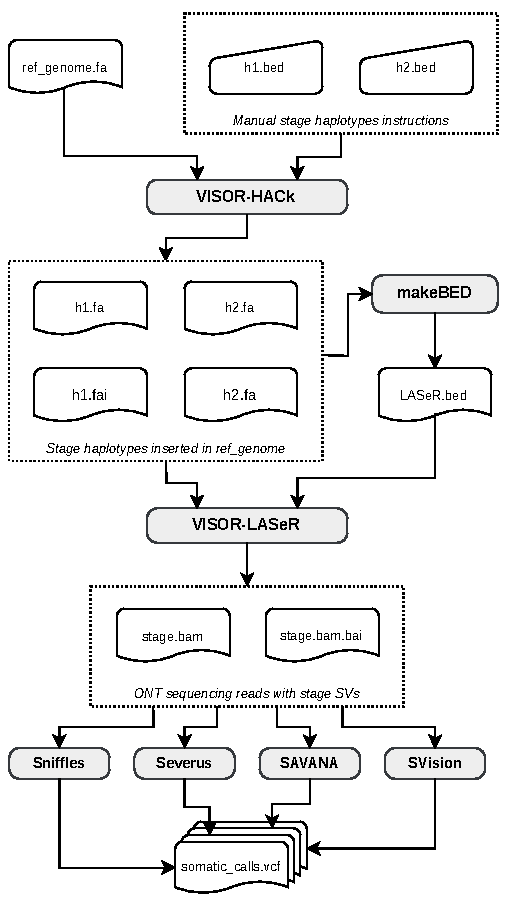
\includegraphics[scale=1.3]{img/visor-simulations.pdf}
    \caption[Simplified version of ``visor-simulations'' workflow for long-read 
    simulation and SV calling]{Simplified version of ``visor-simulations'' 
    workflow for long-read simulation and SV calling. VISOR-HACk generates FASTA 
    files (reference sequences) with incorporated SVs using a reference genome and 
    BED-formatted haplotype instructions (tab-delimited genomic coordinates). 
    The makeBED script creates a BED file (genomic intervals) from maximum 
    chromosome sizes extracted from haplotype FASTAs. VISOR-LASeR then generates 
    BAM files (aligned sequencing reads) and their indexes (.bai) using these 
    files as input. each generating its corresponding variant call file (VCF) 
    containing the identified SVs. The workflow parallelizes simulations 
    across stages using configuration files and wildcards, producing 
    multiple replicates at various sequencing coverages with corresponding 
    normal samples.}
    \label{fig:visor-sim}
\end{figure}

\subsubsection{Simulation stages}

Each stage incorporates specific SVs into the GRCh38 reference genome, simulated 
at four coverage levels: 30x, 50x, 100x, and 200x. The initial stage generated 
one normal sample and three tumor replicates per coverage level, totaling 16 BAM 
simulations. Subsequent stages reused the normal samples, requiring only 12 
simulations each through the automation provided by the ``visor-simulations'' 
workflow. 

The stage generated for this project (v1) incorporated six chromosomal 
aberrations characteristic of multiple myeloma, including tandem duplications, 
deletions, and various types of translocations (\textbf{Table~\ref{tab:stagesV1}}). 
Breakpoint coordinates for these structural variants were approximately 
determined using the UCSC Genome Browser, as specific locations were not 
detailed in the clinical literature.

\begingroup
\vspace{0.35cm}

\footnotesize

\begin{longtable}{>{\RaggedRight\arraybackslash}p{2.5cm} 
                  >{\RaggedRight\arraybackslash}p{10.5cm} 
                  >{\RaggedLeft\arraybackslash}p{1.75cm}}
    \captionsetup{labelfont=bf, font=footnotesize}
    \caption[Simulated chromosomal aberrations characteristic of Multiple 
    Myeloma]{\footnotesize Simulated chromosomal aberrations characteristic of 
    Multiple Myeloma \cite{aksenova_genome_2021}. Size values represent the final 
    length in base pairs (bp) after genome insertion. Tandem duplication 
    consists of a 2,030,586 bp fragment repeated four times. Input files for 
    VISOR read simulation available at 
    \url{https://github.com/villena-francis/visor-simulations/tree/main/resources/v1}}. 
    \label{tab:stagesV1}\\
    
    \toprule
    \rowcolor{lightgray}
    \textbf{SV type} & \textbf{Description} & \textbf{Size (pb)} \\ 
    \midrule
    \endfirsthead
    
    \multicolumn{3}{@{}l}{\RaggedRight \textbf{\tablename\ \thetable{}} -- Continued} \\
    \\
    \toprule
    \rowcolor{lightgray}
    \textbf{SV type} & \textbf{Description} & \textbf{Size (pb)} \\ 
    \midrule
    \\
    \endhead
    \\
    \midrule 
    \multicolumn{3}{r}{\footnotesize Continued on next page} \\
    \endfoot
    
    \bottomrule
    \endlastfoot

    \\
    Tandem \mbox{duplication}         & Amplification of chromosome 1q (1q21+), representing one of the most frequent structural cytogenetic abnormalities in Multiple Myeloma, occurring in approximately 40\% of cases .     & 10152930 \\
    \\
    Deletion                          & Deletion of chromosome 17p, present in approximately 10\% of Multiple Myeloma cases, serves as a significant poor prognostic indicator. The minimally deleted region at locus 17p13 encompasses the tumor suppressor gene TP53 & 234564 \\
    \\
    Translocation \mbox{(reciprocal)} & Chromosomal rearrangement involving the immunoglobulin heavy chain (IGH) gene at 14q32, a hallmark genetic event in Multiple Myeloma pathogenesis.                                                  & 1502367  \\
    \\
    Translocation \mbox{(cut-paste)}  & Rearrangement involving CDKN2A, a crucial tumor suppressor gene whose inactivation through mutations or deletions is among the most frequent alterations in human cancers, second only to TP53 alterations. & 31271 \\
    \\
    Translocation \mbox{(copy-paste)} & Structural variation affecting the KRAS oncogene region, whose alterations are frequently associated with Multiple Myeloma progression.  & 45683 \\
    \\
    Inversion                         & Chromosomal inversion at 6q25.1, included as a control variant to validate the detection capabilities of structural variant analysis pipelines, although not typically characteristic in Multiple Myeloma.          & 3600001  \\
    \\

\end{longtable}
\endgroup

\newpage 

\subsection{Benchmarking of SV callers}

\subsubsection{Data subsampling for local device processing}

Visual inspection of BAM file reads is essential for validating simulation 
quality and SV caller accuracy. Due to cluster limitations with graphical 
interfaces, this analysis requires local processing. We developed a workflow to 
split whole-genome BAM files by chromosome, available at 
\url{https://github.com/villena-francis/bam-splitter}. 
\textbf{Figure \ref{fig:bam-splitter}} illustrates the workflow's key 
components.

\begin{figure}[H]
    \centering
    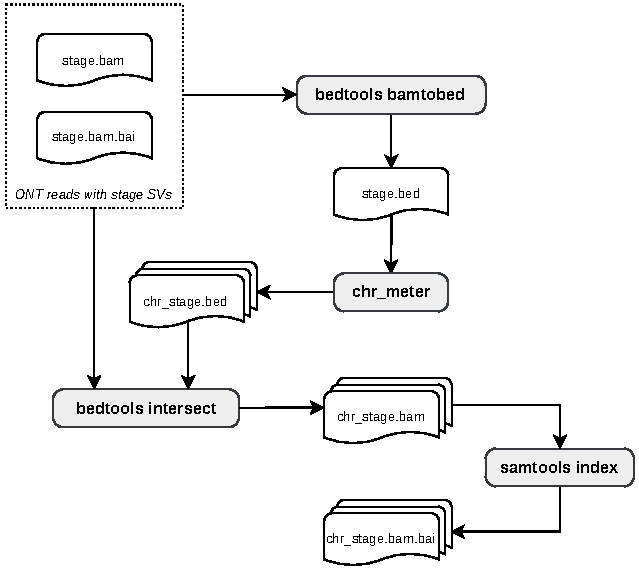
\includegraphics[scale=1.3]{img/bam-splitter.pdf}
    \caption[Simplified version of ``bam-splitter'' workflow for chromosomal 
    splitting of BAM files]{Simplified version of ``bam-splitter'' workflow for 
    chromosomal splitting of BAM files. The process begins with bedtools 
    bamtobed generating a comprehensive BED file of chromosome coordinates. 
    The chr\_meter script then creates individual BED files for selected 
    chromosomes, which bedtools intersect uses to produce chromosome-specific 
    BAM files. Samtools generates corresponding indexes for each BAM file. The 
    workflow employs configuration files and wildcards to parallelize chromosome 
    processing.}
    \label{fig:bam-splitter}
\end{figure}

\subsubsection{Visualization of long read alignments}

Chromosomal BED visualization was conducted using Genome-Wide (GW), an advanced, 
ultra-fast genome browser capable of exploring extensive genomic regions and 
complete chromosomes. GW's specialized features, particularly its VCF-based 
manual curation capability, facilitated rapid validation of SV caller 
predictions.

\subsubsection{Classification of SV calling results}

Performance evaluation of SV callers employed a binary classification framework 
with the following criteria:

\begin{itemize}[label=\tiny\raise.5ex\hbox{•}, leftmargin=\parindent]

    \item \textbf{True Positives (TP)}: Successfully detected simulated SVs.
    
    \item \textbf{False Positives (FP)}: Caller-identified SVs absent in 
    simulation, verified through read inspection.
    
    \item \textbf{False Negatives (FN)}: Simulated SVs present in reads but 
    undetected by caller.

\end{itemize}

True Negatives (TN) were excluded from this analysis due to their 
inapplicability in SV calling evaluation, given the vast genomic space and 
nature of SV detection methods.

\subsubsection{Metrics used}

Due to the impossibility of quantifying true negatives in SV calling, we 
employed TN-independent metrics:

\begin{enumerate}[leftmargin=\parindent]
    
    \item \textbf{Recall}: Proportion of correctly identified positive cases
    \begin{equation}
        \label{eq:recall}
        Recall = \frac{TP}{TP + FN}
    \end{equation}

    \item \textbf{Precision}: Accuracy of positive predictions
    \begin{equation}
        \label{eq:precision}
        Precision = \frac{TP}{TP + FP}
    \end{equation}

    \item \textbf{F1 Score}: Harmonic mean of precision and recall
    \begin{equation}
        \label{eq:f1score}
        F1 = 2 \cdot \frac{precision \cdot recall}{precision + recall}
    \end{equation}

\end{enumerate}

Computational efficiency was evaluated using Slurm-generated statistics: CPU/GPU 
utilization (cores), RAM consumption (GB), and execution time (minutes).

\subsubsection{Data Visualization and Statistical Analysis}

Metric analysis and visualization were implemented through R scripts available 
at \url{https://github.com/villena-francis/master_thesis/tree/main/data/cluster_bmk}.







